\section{mo\-First\-Impr\-Select$<$ M $>$ Class Template Reference}
\label{classmo_first_impr_select}\index{moFirstImprSelect@{moFirstImprSelect}}
One possible {\bf mo\-Move\-Select}{\rm (p.\,\pageref{classmo_move_select})}.  


{\tt \#include $<$mo\-First\-Impr\-Select.h$>$}

Inheritance diagram for mo\-First\-Impr\-Select$<$ M $>$::\begin{figure}[H]
\begin{center}
\leavevmode
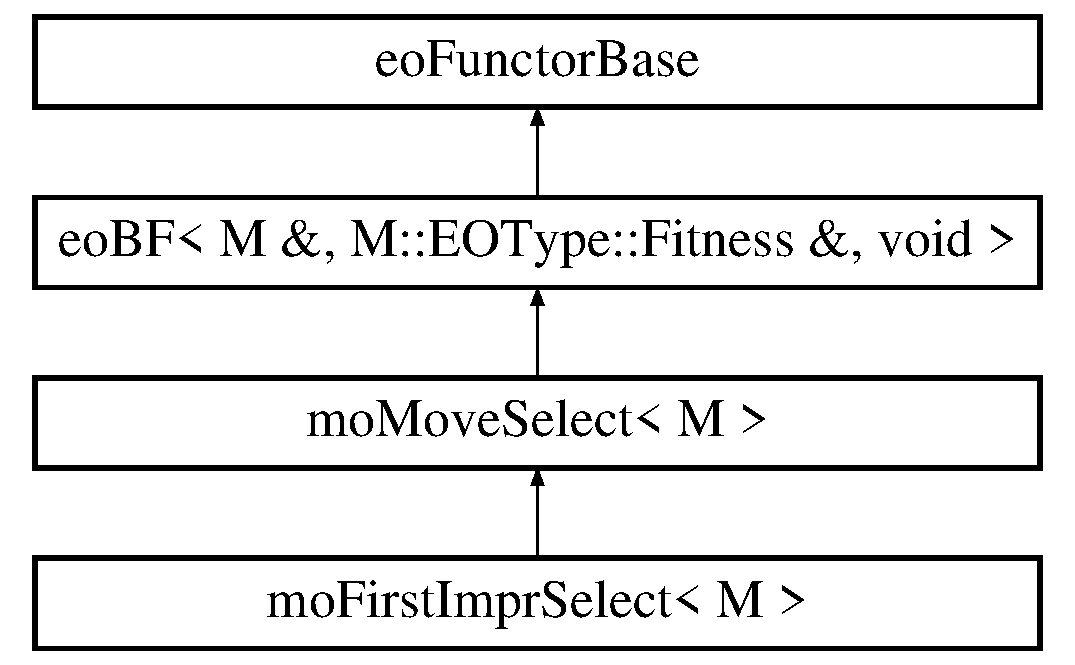
\includegraphics[height=2cm]{classmo_first_impr_select}
\end{center}
\end{figure}
\subsection*{Public Types}
\begin{CompactItemize}
\item 
typedef M::EOType::Fitness {\bf Fitness}\label{classmo_first_impr_select_64763ce3e6d2873266624382b407fa5a}

\begin{CompactList}\small\item\em Alias for the fitness. \item\end{CompactList}\end{CompactItemize}
\subsection*{Public Member Functions}
\begin{CompactItemize}
\item 
virtual void {\bf init} (const {\bf Fitness} \&\_\-\_\-fit)
\begin{CompactList}\small\item\em Procedure which initialise the exploration. \item\end{CompactList}\item 
bool {\bf update} (const M \&\_\-\_\-move, const typename M::EOType::Fitness \&\_\-\_\-fit)
\begin{CompactList}\small\item\em Function that indicates if the current move has not improved the fitness. \item\end{CompactList}\item 
void {\bf operator()} (M \&\_\-\_\-move, {\bf Fitness} \&\_\-\_\-fit)  throw (Empty\-Selection)
\begin{CompactList}\small\item\em Procedure which saved the best move and fitness. \item\end{CompactList}\end{CompactItemize}
\subsection*{Private Attributes}
\begin{CompactItemize}
\item 
bool {\bf valid}\label{classmo_first_impr_select_a99c0586ba07449234705c17a258d58c}

\begin{CompactList}\small\item\em Allow to know if at least one move has improved the solution. \item\end{CompactList}\item 
M {\bf best\_\-move}\label{classmo_first_impr_select_dfed419a608dd7c41f07fa1f1279cb8c}

\begin{CompactList}\small\item\em Best stored movement. \item\end{CompactList}\item 
{\bf Fitness} {\bf init\_\-fit}\label{classmo_first_impr_select_ce7ba63e8cc3a9164f4e546477e98ca8}

\begin{CompactList}\small\item\em Initial fitness. \item\end{CompactList}\item 
{\bf Fitness} {\bf best\_\-fit}\label{classmo_first_impr_select_e1190347b76ec6fe717be32354b4a9a9}

\begin{CompactList}\small\item\em Best stored fitness. \item\end{CompactList}\end{CompactItemize}


\subsection{Detailed Description}
\subsubsection*{template$<$class M$>$ class mo\-First\-Impr\-Select$<$ M $>$}

One possible {\bf mo\-Move\-Select}{\rm (p.\,\pageref{classmo_move_select})}. 

The neighborhood is explored until a move enables an improvment of the current solution. 



Definition at line 23 of file mo\-First\-Impr\-Select.h.

\subsection{Member Function Documentation}
\index{moFirstImprSelect@{mo\-First\-Impr\-Select}!init@{init}}
\index{init@{init}!moFirstImprSelect@{mo\-First\-Impr\-Select}}
\subsubsection{\setlength{\rightskip}{0pt plus 5cm}template$<$class M$>$ virtual void {\bf mo\-First\-Impr\-Select}$<$ M $>$::init (const {\bf Fitness} \& {\em \_\-\_\-fit})\hspace{0.3cm}{\tt  [inline, virtual]}}\label{classmo_first_impr_select_4c5ce18ede46247a439c68f6954a4055}


Procedure which initialise the exploration. 

It save the current fitness as the initial value for the fitness. 

Implements {\bf mo\-Move\-Select$<$ M $>$} {\rm (p.\,\pageref{classmo_move_select_bca4c43f13d26eca7163aeb272a4a52e})}.

Definition at line 35 of file mo\-First\-Impr\-Select.h.

References mo\-First\-Impr\-Select$<$ M $>$::init\_\-fit, and mo\-First\-Impr\-Select$<$ M $>$::valid.\index{moFirstImprSelect@{mo\-First\-Impr\-Select}!update@{update}}
\index{update@{update}!moFirstImprSelect@{mo\-First\-Impr\-Select}}
\subsubsection{\setlength{\rightskip}{0pt plus 5cm}template$<$class M$>$ bool {\bf mo\-First\-Impr\-Select}$<$ M $>$::update (const M \& {\em \_\-\_\-move}, const typename M::EOType::Fitness \& {\em \_\-\_\-fit})\hspace{0.3cm}{\tt  [inline]}}\label{classmo_first_impr_select_7ba0882728daedc75c249647c070ccf0}


Function that indicates if the current move has not improved the fitness. 

If the given fitness enables an improvment, the move ({\bf mo\-Move}{\rm (p.\,\pageref{classmo_move})}) should be applied to the current solution.

\begin{Desc}
\item[Parameters:]
\begin{description}
\item[{\em \_\-\_\-move}]a move. \item[{\em \_\-\_\-fit}]a fitness linked to the move. \end{description}
\end{Desc}
\begin{Desc}
\item[Returns:]TRUE if the move does not improve the fitness. \end{Desc}


Definition at line 52 of file mo\-First\-Impr\-Select.h.

References mo\-First\-Impr\-Select$<$ M $>$::best\_\-fit, mo\-First\-Impr\-Select$<$ M $>$::best\_\-move, mo\-First\-Impr\-Select$<$ M $>$::init\_\-fit, and mo\-First\-Impr\-Select$<$ M $>$::valid.\index{moFirstImprSelect@{mo\-First\-Impr\-Select}!operator()@{operator()}}
\index{operator()@{operator()}!moFirstImprSelect@{mo\-First\-Impr\-Select}}
\subsubsection{\setlength{\rightskip}{0pt plus 5cm}template$<$class M$>$ void {\bf mo\-First\-Impr\-Select}$<$ M $>$::operator() (M \& {\em \_\-\_\-move}, {\bf Fitness} \& {\em \_\-\_\-fit})  throw ({\bf Empty\-Selection})\hspace{0.3cm}{\tt  [inline]}}\label{classmo_first_impr_select_3be12cf4cbaed00df7c4fa735b2c0a95}


Procedure which saved the best move and fitness. 

\begin{Desc}
\item[Parameters:]
\begin{description}
\item[{\em \_\-\_\-move}]the current move (result of the procedure). \item[{\em \_\-\_\-fit}]the current fitness (result of the procedure). \end{description}
\end{Desc}
\begin{Desc}
\item[Exceptions:]
\begin{description}
\item[{\em {\bf Empty\-Selection}{\rm (p.\,\pageref{class_empty_selection})}}]if no move has improved the fitness. \end{description}
\end{Desc}


Definition at line 76 of file mo\-First\-Impr\-Select.h.

References mo\-First\-Impr\-Select$<$ M $>$::best\_\-fit, mo\-First\-Impr\-Select$<$ M $>$::best\_\-move, and mo\-First\-Impr\-Select$<$ M $>$::valid.

The documentation for this class was generated from the following file:\begin{CompactItemize}
\item 
mo\-First\-Impr\-Select.h\end{CompactItemize}
